% This is "sig-alternate.tex" V2.0 May 2012
% This file should be compiled with V2.5 of "sig-alternate.cls" May 2012
%
% This example file demonstrates the use of the 'sig-alternate.cls'
% V2.5 LaTeX2e document class file. It is for those submitting
% articles to ACM Conference Proceedings WHO DO NOT WISH TO
% STRICTLY ADHERE TO THE SIGS (PUBS-BOARD-ENDORSED) STYLE.
% The 'sig-alternate.cls' file will produce a similar-looking,
% albeit, 'tighter' paper resulting in, invariably, fewer pages.
%
% ----------------------------------------------------------------------------------------------------------------
% This .tex file (and associated .cls V2.5) produces:
%       1) The Permission Statement
%       2) The Conference (location) Info information
%       3) The Copyright Line with ACM data
%       4) NO page numbers
%
% as against the acm_proc_article-sp.cls file which
% DOES NOT produce 1) thru' 3) above.
%
% Using 'sig-alternate.cls' you have control, however, from within
% the source .tex file, over both the CopyrightYear
% (defaulted to 200X) and the ACM Copyright Data
% (defaulted to X-XXXXX-XX-X/XX/XX).
% e.g.
% \CopyrightYear{2007} will cause 2007 to appear in the copyright line.
% \crdata{0-12345-67-8/90/12} will cause 0-12345-67-8/90/12 to appear in the copyright line.
%
% ---------------------------------------------------------------------------------------------------------------
% This .tex source is an example which *does* use
% the .bib file (from which the .bbl file % is produced).
% REMEMBER HOWEVER: After having produced the .bbl file,
% and prior to final submission, you *NEED* to 'insert'
% your .bbl file into your source .tex file so as to provide
% ONE 'self-contained' source file.
%
% ================= IF YOU HAVE QUESTIONS =======================
% Questions regarding the SIGS styles, SIGS policies and
% procedures, Conferences etc. should be sent to
% Adrienne Griscti (griscti@acm.org)
%
% Technical questions _only_ to
% Gerald Murray (murray@hq.acm.org)
% ===============================================================
%
% For tracking purposes - this is V2.0 - May 2012

\documentclass[10pt]{report}
\usepackage{hyperref}
\usepackage{graphicx}
\usepackage{pdfpages}
\usepackage{appendix}

\usepackage[margin=1.2in]{geometry}
\hypersetup{
    colorlinks=false,
    pdfborder={0 0 0},
}
\begin{document}



% TITLE PAGE
\begin{titlepage}

\begin{center}

\textup{\large Major Project}\\[1.0cm]

% Title
\uppercase{\Large \textbf {EXPERIMENTAL OPERATING SYSTEM}}\\[3.0cm]

% Done by

\begin{table}[h]
\centering
\begin{tabular}{lr}\hline \\
B090084CS & Shamil CM \\
B090066CS & Sreeraj S \\ 
B090468CS & Vivek Anand T Kallampally \\ \\ \hline 
\end{tabular}
\end{table}

\vspace{2cm}

\large \textit{Under the guidance of} \\
\large \textbf{Dr. K. Muralikrishnan}

\vfill

% Bottom of the page

\includegraphics[width=0.20\textwidth]{./nitc-logo}\\[1cm]
\large{DEPARTMENT OF COMPUTER SCIENCE AND ENGINEERING}\\
\normalsize
\textsc{National Institute of Technology Calicut}\\
Calicut, Kerala 673 601 \\
\vspace{0.5cm}


\end{center}

\end{titlepage}
%
% --- Author Metadata here ---

%\CopyrightYear{2007} % Allows default copyright year (20XX) to be over-ridden - IF NEED BE.
%\crdata{0-12345-67-8/90/01}  % Allows default copyright data (0-89791-88-6/97/05) to be over-ridden - IF NEED BE.
% --- End of Author Metadata ---

%\title{XOS : Experimental Operating System }

%
% You need the command \numberofauthors to handle the 'placement
% and alignment' of the authors beneath the title.
%
% For aesthetic reasons, we recommend 'three authors at a time'
% i.e. three 'name/affiliation blocks' be placed beneath the title.
%
% NOTE: You are NOT restricted in how many 'rows' of
% "name/affiliations" may appear. We just ask that you restrict
% the number of 'columns' to three.
%
% Because of the available 'opening page real-estate'
% we ask you to refrain from putting more than six authors
% (two rows with three columns) beneath the article title.
% More than six makes the first-page appear very cluttered indeed.
%
% Use the \alignauthor commands to handle the names
% and affiliations for an 'aesthetic maximum' of six authors.
% Add names, affiliations, addresses for
% the seventh etc. author(s) as the argument for the
% \additionalauthors command.
% These 'additional authors' will be output/set for you
% without further effort on your part as the last section in
% the body of your article BEFORE References or any Appendices.



% There's nothing stopping you putting the seventh, eighth, etc.
% author on the opening page (as the 'third row') but we ask,
% for aesthetic reasons that you place these 'additional authors'
% in the \additional authors block, viz.
%\date{30 July 1999}
% Just remember to make sure that the TOTAL number of authors
% is the number that will appear on the first page PLUS the
% number that will appear in the \additionalauthors section.

%\maketitle

%CERTIFICATE

\newpage
\thispagestyle{empty}

\begin{center}

\LARGE{Department of Computer Science and Engineering}\\
\normalsize
\textsc{National Institute of Technology Calicut}\\[2.0cm]

\emph{\LARGE Certificate}\\[2.5cm]
\end{center}
\normalsize This is to certify that this is a bonafide record of the project presented by the students whose names are given below during Winter 2013 in partial fulfilment of the requirement of the course of B.Tech Computer Science and Engineering.\\[1.0cm]

\begin{table}[h]
\centering
\begin{tabular}{lr}
\hline
\\
B090084CS & Shamil CM \\ 
B090066CS & Sreeraj S \\
B090468CS & Vivek Anand T Kallampally \\
\\
\hline
\end{tabular}
\end{table}

\vfill


% Bottom of the page
\begin{flushright}
Faculty In-charge\\[1.5cm]
Course Co-ordinator\\[1.0cm]
\end{flushright}

\begin{flushleft}
Date:
\end{flushleft}



% ABSTRACT
\begin{abstract}
This paper introduces an operating system project that helps undergraduate computer science students acquire an elementary understanding of the practical aspects of an operating system. The specification of XOS (Experimental Operating System) has been laid out for students to build it from scratch in a bottom-up manner. XOS runs on a simulated machine hardware with a very simple  instruction set  and native filesystem. Unlike other common instructional operating systems, the complete development environment including custom programming languages, debugger, file system interface and a detailed implementation roadmap is provided. 

\end{abstract}

% A category with the (minimum) three required fields

\pagenumbering{roman} %numbering before main content starts
\tableofcontents

\newpage
\pagenumbering{arabic}




\chapter{Introduction}

Teaching operating systems has been a challenge at the undergraduate level. To tackle this problem several instructional operating systems like Nachos\cite{nachos}, OS/161\cite{os161}, Pintos\cite{Pintos}, \\GeekOS \cite{survey} etc. have been developed by various universities. Nachos\cite{nachos} has been one of the most popular instructional operating systems available and is being used in many institutes across the world \cite{survey}. Implementing Nachos is simple and it uses a mixed mode approach, where the operating system kernel is co-resident with the machine simulator and fused together as a single program. Nachos\cite{nachos} and OS/161\cite{os161} runs on top of MIPS machine simulator. For these systems, a user's machine running on other platforms require cross compilers to MIPS. \\

 
Instructional operating systems like Minix and Xinu \cite{survey}, provide a functional operating system on which modifications are to be done by students. Almost every other instructional operating system provides a skeleton of an operating system. However in XOS, only the specification has been laid out, and students learn to implement XOS from ground up using the tools provided. In this project, a simple high level language called APL (Application Programmer's Language) and its cross-compiler to XSM instruction set is provided to write user programs to test XOS. An XSM dependent language called SPL (System Programmers Language) and its cross-compiler is provided to program the OS itself. Most instructional operating systems use the UNIX filesystem for file management by the operating system. Instead, XOS provides a native file system known as XFS (Experimental File System). An interface between the UNIX filesystem and XFS filesystem is also provided.  \\

XOS has features like multiprogramming, process management, a primitive  filesystem and virtual memory. A sequence of stages are provided in a detailed roadmap which helps students to build XOS sequentially. Several simplifications have been made in XOS specification to make the system simple and manageable as a short-term project. These include absence of inter-process communication, device management, file caching, file permissions etc.  Only the fundamental data structures and functions of a single-user, multiprogramming operating system has been retained. Limited support for process synchronization can be added to XOS as enhancements (refer section \ref{sec:roadmap}). The features that are omitted from XOS are not intended to be done in this platform. The project has been designed to provide an essential understanding of operating system concepts for a student undertaking a core theory course in  operating systems at undergraduate level. XOS is not scalable and students intending to go in depth in topics like device management, file caching etc. are suggested to move on to more sophisticated platforms like Minix, GeekOS\cite{survey} etc. \\

In our experience with Nachos at junior year undergraduate operating systems laboratory course, we observed that students did not have the necessary programming expertise to comprehend the large code base of Nachos.  We also observed that students faced a conceptual difficulty in understanding the separation between the operating system kernel and the machine simulator which are fused together as a single program in Nachos. XOS addresses these issues by allowing the student to build the operating system from scratch without having to learn an existing code base. The roadmap is designed in such a way that the student can read the roadmap and complete the project without any supervision. The project is expected to provide the student with a better insight into the operating systems concepts described in standard text books like \cite{silberschatz}. Building XOS can be a supplementary project for a junior level undergraduate course in operating systems spanning over a 12 to 16 week term. \\




\chapter{Components}

\section{Introduction}
The primary components of the project include a simulated machine hardware (XSM), file system (XFS) and the operating system (XOS). No code base for the operating system is provided and the operating system is completely implemented by the student. Apart from the primary components, various tools are provided as part of the development environment. They include languages like Application Programmer's Language (APL) and System Programmer's Language (SPL) and their cross compilers to XSM instruction set, XSM debugger, and a UNIX-XFS interface to transfer files between a UNIX machine and the XFS disk (the XFS disk is itself a UNIX file). 

\begin{figure}[hbtp]
\centering
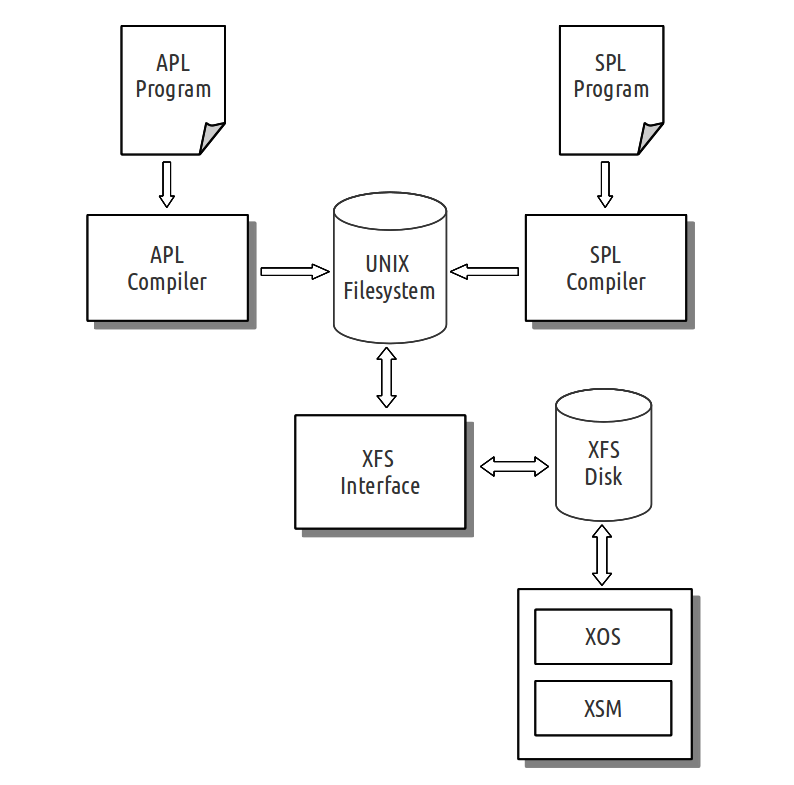
\includegraphics[scale=0.4]{components.png}
\caption{Components and their interaction}
\end{figure}



\section{Experimental File System }
The disk for XSM (which is a UNIX file) can be formatted using XFS or Experimental File System. XFS is the file system compatible with XOS. Since file system management is done by students building XOS, the disk organization must be easily understood and at the same time must give an insight on the data structures used in real file systems. Hence we chose to have a native file system for XOS.\\

The disk is formatted with this file system using the interface provided as part of the development environment. XFS is a simple file system with no directory structure. The data is organized into blocks of size equal to the page size in XSM memory. There are 512 blocks in XFS which holds the file and disk data structures, OS routines, user programs and data files. The various data structures in XFS include the Disk Free List which maintains information about used and unused blocks on the disk and the FAT or the File Allocation Table stores details of the files in the disk.



\section{Experimental String Machine }
XOS runs on a simulated machine hardware called XSM or Experimental String Machine. XSM uses an easy-to-understand native 2-address instruction set. The various components of the machine include registers, memory, timer and the disk. A UNIX file simulates the disk for XSM.\\

XSM has a timer which triggers after fixed number of instructions as compared to a timer interval in real machines. An instruction triggered timer was preferred over a clock-triggered timer to ensure that the timer interrupt is not invoked in between the simulation of a single instruction. Thus, an instruction in XSM is always atomic. Instructions are executed one after the other in a non-pipelined manner.\\

XSM has a memory of 64 pages. Size of each page is 512 words. A word is the smallest addressable unit in XSM as compared to a byte in MIPS. XSM is a string machine, and each word is stored internally as strings of size 16 characters.  However, the XSM supports two data types, integer and strings and has instructions for both  the data types. There are two privilege modes in XSM, the user mode and kernel mode. Switching between modes is done by instructions.\\

XSM instruction set supports load and store instructions to load data from the disk to memory and to store data from memory to disk respectively. Real machines usually implement transfer using a DMA (Direct Memory Access) controller which transfers data directly between disk and memory and signals the processor after the transfer is complete. This happens without intervention of the processor. However XSM, provides machine instructions to do this. It is a deviation from real machines and has been provided to avoid the complexity associated with device management by the operating system when more than one process is running. We decided to avoid device management and DMA altogether because it is beyond the scope of the project. We feel that such features may be attempted on more advanced platforms like Minix after the completion of this project. \\

XSM supports virtual memory management. The machine will transfer control to a specified location in memory where the exception handler is expected to reside upon encountering an exception after setting an EFR or the Exception Flag Register. Unlike MIPS machines\cite{mips}, which has 3 registers for exception handling, XSM combines all three registers into a single register for simplicity. Exceptions in XSM include a page fault, illegal instructions or operands, illegal memory access and arithmetic exceptions. \\

XSM machine has capability of running an operating system capable of multiprogramming, file management and virtual memory on top of it. XOS has been designed to exploit the complete capabilities of the XSM architecture, keeping in mind a simplistic design. The motivation behind the design of all components was sequentially building the concepts of operating systems and not on the intricate details associated with its implementation.




\section{Experimental Operating System }

\begin{figure}[hbtp]
\centering
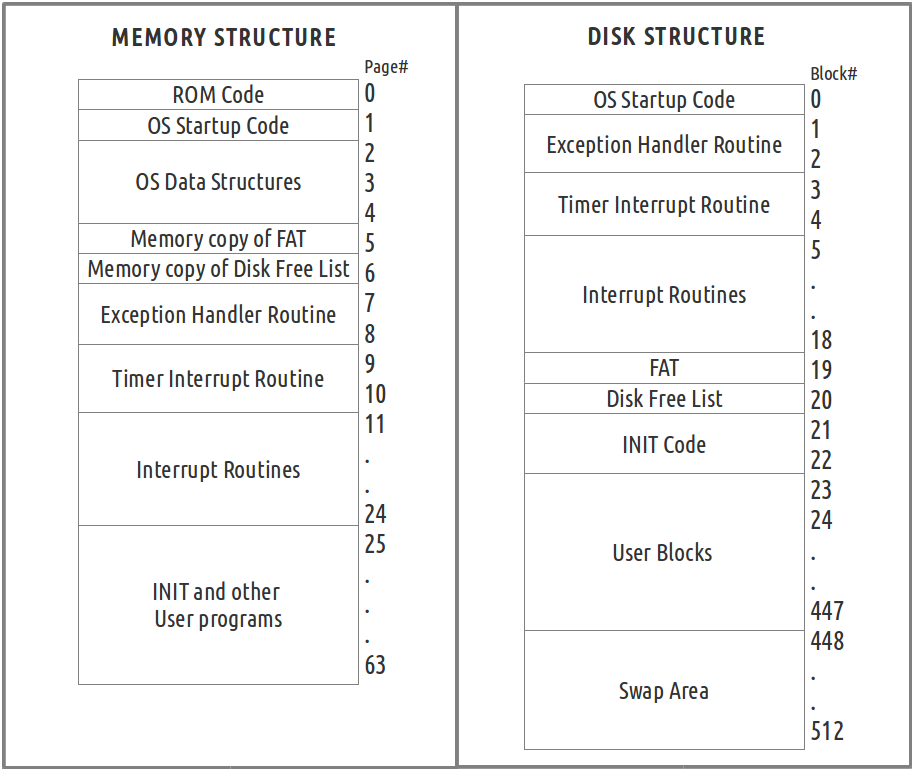
\includegraphics[scale=0.35]{memdiskstructure.png}
\caption{OS View of memory and disk}
\end{figure}

The specification for an Experimental Operating System or XOS is provided to the students. In this project, students will build XOS to meet the specification. XOS is a simulated operating system which runs on top of XSM which is a simulated machine hardware. The OS kernel unlike Nachos \cite{nachos} resides in the memory of the simulated machine. The disk for XOS, which is a UNIX file,  is formatted with the XFS filesystem. The disk permanently stores the OS routines and data structures as in real systems.  \\

The various components of the operating system include routines like OS startup code, eight interrupt routines including the timer interrupt, the exception handler routine, and data structures like ready list of PCBs, per-process page tables, the system wide-open file table, memory free list, memory copy of disk data structures including FAT and the disk free list. The OS routines are to be programmed by the student building XOS and is loaded to the disk. The OS startup code which is also programmed by the student is responsible for loading all the other routines from disk to memory on OS startup. The OS startup code must be loaded in the first block of the XFS disk. When the system boots the bootstrap loader or the ROM code will copy this disk block to memory and pass control to it. The ROM code is hardcoded in the part of the machine memory which acts as the ROM. The OS routines will modify the memory-resident data structures, and make changes in the disk as and when required. \\


\begin{figure}[hbtp]
\centering
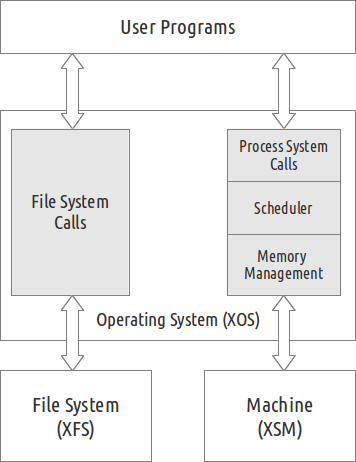
\includegraphics[scale=0.55]{xosstructure.png}
\caption{Components and their interaction}
\end{figure}


The various functionalities of XOS are process management, memory management and system calls. Process management includes scheduling and dispatching processes to the CPU. XOS is capable of multiprogramming (the ability to run more than one process simultaneously). Memory Management involves allocating memory for processes, demand paging (loading memory pages from the disk as and when required). The system calls provided by XOS include file system calls like Create, Delete, Open, Close, Read, Write, Seek and process system calls like Fork, Exec and Exit. Limited support for process synchronization has been suggested in the form of enhancements to XOS, through the implementation of system calls like Wait, Signal, Getpid, and Getppid. These system calls are mapped to 7 interrupt routines provided by the machine. The scheduler should be programmed and loaded into the timer interrupt routine. By specification, the scheduler of XOS follows a round-robin scheduling technique \cite{silberschatz}. The page fault handler resides in the exception handler routine. For exceptions other than the page fault, XOS will exit the process. On a page fault exception, the exception handler must be programmed to implement a page replacement algorithm. The page replacement algorithm in XOS specification is the \textit{second chance algorithm}\cite{silberschatz} \\

XOS maintains a ready list of PCBs in memory. XOS limits the number of processes that can be run concurrently to 32. Each process has a per-process page table in memory. For each process the stack is of size 1 page and is present in the memory always. A process can have a maximum of 4 memory pages. Even though space for 32 processes to reside simultaneously in memory is not available, with pure demand paging, and swapping out of pages by the page replacement algorithm, this constraint can be overcome. The stack is never swapped out to the disk. When a OS routine returns back to the user program,  the stack of the user process is used for passing the return address. \\

No code base for XOS is presented to the student. However a detailed roadmap which is divided into well-defined stages is provided so that the student can both understand the concepts and build the operating system to meet the specification.




\chapter{Development Tools}

Various development tools are provided to the student for implementing XOS. Each of these tools and their purpose is described in the following sections. 


\section{Application Programmer's Language}
Application Programmer's Language (APL) is a high-level language which can be used to write application programs to run on top of XOS. Its cross-compiler to XSM instruction set is provided as part of the development tools to the student. APL is a simple language which supports local and global variables and function calls. Interfaces to XOS system calls are provided through a family of built-in functions. \\


\section{System Programmer's Language}
System Programmer's Language (SPL) is a XSM dependent language which is used to program XOS itself. Its cross-compiler to XSM instruction set is also provided as part of the development tools. SPL unlike APL, is close to the machine instruction set. SPL statements can access most of the machine registers and memory directly. SPL has predefined constants specific to XOS. The SPL programmer can redefine these constants or define new constants. Apart from this, XOS provides \textit{aliasing}, when registers can be assigned meaningful names for convenience.\\


\section{Debugger}
The XSM simulator can be run in the debug mode. In this mode, the machine will stop execution at predefined breakpoints in the XSM instructions loaded in the machine's memory. Breakpoints can be set through APL and SPL programs using the \texttt{breakpoint} instruction. From a breakpoint onwards, the execution can be single stepped, or continued to the next breakpoint in the debugger. Using the debugger, contents of registers, memory, XOS data structures etc, can be verified. The debugger has been modeled based on the GNU Debugger \cite{gdb}.\\


\section{XFS Interface}
The XFS disk is a UNIX file. XFS interface is a simple command-line interface that helps access this disk directly from your UNIX machine. XFS interface has functions to format the disk, display the contents of the disk, copy files from UNIX machine to the disk, view the disk free list etc. The OS routines and user programs are loaded to the disk before starting the OS using this interface.\\

\chapter{Roadmap}
\label{sec:roadmap}
We felt the necessity for a roadmap to build XOS sequentially. A detailed roadmap divided into stages is provided on the onset to help students do the project. The first two stages help students get familiarized with the environment and development tools. Then the students sequentially start running a kernel program and then a user program on top of it. The next big step in the roadmap is when the student starts to run multiple programs and implements the scheduler. The initial stages are explained in detail. The students will learn more than what they do in these stages. The later stages include implementing the system calls, and virtual memory management. The final stage of the roadmap includes making a console for XOS. The entire roadmap is designed so that the project can be completed in a 12 to 16 week term. Moreover, instructions to implement enhancements to XOS which include system calls like Wait, Signal, Getpid, and Getppid and making a console for XOS are provided at the end of the roadmap. These system calls provide limited support for implementing process synchronization. \\

\chapter{Conclusions}
The project is easier to implement compared to the existing instructional operating system due to the simplifications done, and the documentation. The project aims to be a better tool for basic undergraduate understanding of operating systems as it helps students get a feel of the elementary practical aspects of operating systems. It acts as a tool which will aid students to better comprehend the textbooks on operating systems or move on to a complex operating system platform later.


%%ACKNOWLEDGMENTS are optional
\section{Acknowledgments}
We thank the past contributers of the earlier versions of this project, Ajeet Kumar, Albin Suresh, Avinash, Deepak Goyal, Jeril K George, K Dinesh, Mathew Kumpalamthanam, Naseem Iqbal, Nitish Kumar, Ramnath Jayachandran, Sathyam Doraswamy, Sumesh B and Yogesh Mishra. We also thank Govind Nharekat and Nithin Mohan who are undergraduate computer science students at our institute, who were actively involved in testing out the system and providing valuable feedback. 


\section{Availability}
The complete set of development tools, specification documents and roadmap is available at \url{xosnitc.github.com}. The entire source code is hosted at \url{http://github.com/xosnitc}. Students doing XOS project can join the mailing list \url{xos-users@googlegroups.com} and post queries.


\bibliographystyle{abbrv}
\bibliography{report}  % sigproc.bib is the name of the Bibliography in this case
% You must have a proper ".bib" file
%  and remember to run:
% latex bibtex latex latex
% to resolve all references
%
% ACM needs 'a single self-contained file'!
%

\begin{appendices}
\chapter{Operating System (XOS) Specification }
\includepdf[pages={2-}]{../xos/xos.pdf}
\chapter{Machine (XSM) Specification }
\includepdf[pages={2-}]{../xsm/xsm.pdf}
\chapter{Filesystem (XFS) Specification }
\includepdf[pages={2-}]{../xfs/xfs.pdf}
\chapter{Application Programmer's Language (APL) Specification}
\includepdf[pages={2-}]{../apl/apl.pdf}
\chapter{System Programmer's Language (SPL) Specification}
\includepdf[pages={2-}]{../spl/spl.pdf}
\end{appendices}




\end{document}
